\section{Theoretical Foundations}\label{Sec:Method}

In this section we provide a brief introduction into covariate shift and illustrate, how it can be related to credit scoring. In the subsections below, we will then explore the lattice regression framework and its monotonicity and calibration extensions.

\subsection{Covariate Shift}\label{Sec:covshift}

In supervised machine learning, it is often assumed that the test and training data follow the same distributions, or that it does not matter if their domains do not match. In real-world applications this mismatch can lead to models performing well in a certain context, but failing in other contexts, where, compared to the training context, the data shifted. Data set shift therefore describes the effects of the violation of the above mentioned assumption. In the literature there are several approaches to systemize data set shift: \citep{storkey2009training} describes causes of data set shift, \citep{moreno2012unifying} systemize four different effect types of shift (the three types stated in Sec. \ref{Sec:intro} plus `other types') and \citep{kull2014patterns} refine the aforementioned approaches by extending the categorization and by supplementing it with a formal notation using graphical models. For our purpose it will be sufficient to refer to the simple distinction of shifts as described by Moreno-Torres et al., as the specifications of Kull and Flach concern relatively particular cases. 

\citep{moreno2012unifying} model dataset shift as a change in the joint probability distribution $P(y,x)$ of the covariates $X$ and the labels $Y$: 
\begin{quote}
	{\it \textbf{Dataset shift} appears when training and test joint distributions are different. That is, when $P_{tr}(y,x) \neq P_{tst}(y,x)$.}
\end{quote}

The authors give a further specification of the joint distribution $P(y,x)$ to take into consideration the causal relationship between covariates and class labels. The kind of shift that is possible depends on the structure of the problem, leading to the distinction of two cases: for $X \rightarrow Y$ problems values of covariates causally determine the class label; for $Y \rightarrow X$ problems class labels determine the values of covariates. For the former the joint probability distribution $P_{tr}(y,x) = P_{tst}(y,x)$ can then be written as $P(y|x)P(x)$, for the later as $P(x|y)P(x)$. 

From the above Moreno-Torres et al. obtain a formal definition of covariate shift:
\begin{quote}{ \it
	\textbf{Covariate shift} appears only in $X \rightarrow Y$ problems, and is defined as the case where $P_{tr}(y|x) = P_{tst}(y|x)$  and $P_{tr}(x) \neq P_{tst}(x)$.}
\end{quote}
Here only the distributions of $x$ for test and train sets change, the functional relationship of the model stays the same. For a mathematical more rigorous description of the entire problem setting see \citep{sugiyama2012machine}. The definitions of the other types of shift are summarized in Tab. \ref{Tab:dataset_shift}. 

\begin{table}[ht]
	\begin{center}
		{\footnotesize
			\begin{tabular}{lcccc}
%				\toprule
%				& $X \rightarrow Y$ Problem & & $Y \rightarrow X$ Problem & \\
%				\hline
%				& $P_{tr}(y|x) = P_{tst}(y|x)$ & $P_{tr}(x) = P_{tst}(x)$    & $P_{tr}(x|y) = P_{tst}(x|y)$     & $P_{tr}(y) = P_{tst}(y)$  \\
%				\hline
				\toprule
				\multicolumn{1}{c}{ } & \multicolumn{2}{c}{$X \rightarrow Y$ Problem} & \multicolumn{2}{c}{$Y \rightarrow X$ Problem } \\
				\cmidrule(l{3pt}r{3pt}){2-3} \cmidrule(l{3pt}r{3pt}){4-5} 
				& $P_{tr}(y|x) = P_{tst}(y|x)$ & $P_{tr}(x) = P_{tst}(x)$    & $P_{tr}(x|y) = P_{tst}(x|y)$     & $P_{tr}(y) = P_{tst}(y)$  \\
				\midrule
				Covariate Shift   & True & False & -- & --   \\
				Prior Probability Shift  & -- & -- & True & False \\
				Concept Shift & False & True & False & True\\
				Other types & False & False & False &False \\
				\bottomrule
		\end{tabular}}
	\end{center}
	\caption{The four types of dataset shift displayed in form of a logical truth table for both kinds of problem. Each depicted case leads to $P_{tr}(y,x) \neq P_{tst}(y,x)$.} 
	\label{Tab:dataset_shift}
\end{table}



To illustrate the relationship between covariate shift and credit scoring we draw on an example from \citep[Sec.~8.2]{wang2020deontological}. Here, a credit scoring model is employed based on the Taiwanese UCI Credit Card data set, which we also will use for our experiment in Sec. \ref{Sec:Exp}. The authors remark a potenital bias for the variable `Repayment status (April)', as the data appears to be very noisy for cases with $overdue > 3$ (see Appendix Fig. \ref{Fig:gup3}). In a simplified two-feature test case (with covariates `Marital status' and `Repayment status (April)') their model then yields the output visualized in Fig. \ref{Fig:gup2}:

\begin{figure}[htb!]
	\centering
	\begin{minipage}{0.45\textwidth}
		\centering
		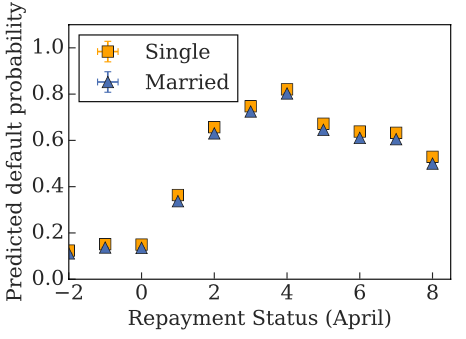
\includegraphics[width=1\textwidth]{img/gup2} % first figure itself
		\caption{Baseline model}
		\label{Fig:gup2}
	\end{minipage}\hfill
	\begin{minipage}{0.45\textwidth}
		\centering
		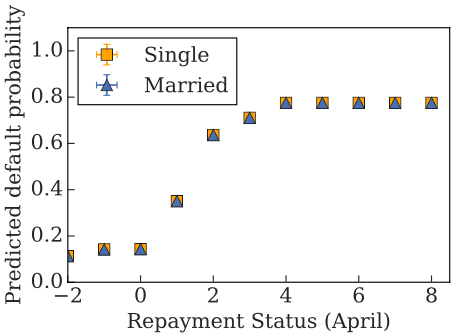
\includegraphics[width=1\textwidth]{img/gup1} % second figure itself
		\caption{Lattice model}
		\label{Fig:gup1}
	\end{minipage}
\end{figure}

Fig. \ref{Fig:gup2} shows that customers who are 5 or 6 month overdue, are assigned a lower score than those, who are only 2 months overdue. This means, borrowers are penalized by the score for paying back in time. The underlying bias most likely results from the training data only containing 122 cases of $overdue > 3$, leaving those cases underrepresented in a training set of 30.000 observations. We can then model this example as a case of covariate shift.  

Assume we now want to apply the classifier in a new context. In our new test set there is a significantly higher amount of observations with $overdue > 3$ for `April repayment', let it be 5\% instead of 0.4\%. We then have $P_{tr}(\mathrm{April\ repayment}) \neq P_{tst}(\mathrm{April\ repayment})$, potentially penalizing those customers who are only slightly overdue. All other variables fixed, those customers obtain a worse credit score then heavy overdue customers. The functional relationship $P(y|x)$ remains unchanged, but the input distribution $p(x)$ differs. 

To mitigate the bias of the estimator, Wang and Gupta supplement their lattice model with a \textit{mononicity shape constraint}. In Fig. \ref{Fig:gup1} we see a more consistent behaviour of the estimator, as the shape constraint permits to integrate prior knowledge into the model. For their experiment the authors used a nonlinear generalized additive model, respectively a TFL calibrated linear model. In the following subsections we explore the concept behind the lattice modeling approach.

\subsection{Lattice Regression}

\textit{Lattice regression} is the name for a regression method, in which the estimated function is represented as a rectangular grid of function values spanning the input domain. As in a textbook lookup table for the $z$-values of standard normal distribution, any needed value can then be linearly interpolated from the lattice. In developing supervised machine learning applications we usually start from scratch fitting a function $f(x)$ to the available training data by using some regression algorithm, with the data consisting of randomly sampled pairs $\{(x_i, y_i)\}$. In a second step $f(x)$ can then be evaluated on a lattice to generate a look up table. There is a disadvantage to this two-step procedure, though, as the effect of interpolation from the lattice nodes (on the error of the training samples) is not taken into account, respectively the empirical risk function does not consider the interpolation step. To solve this issue, \citep[pp.~1]{garcia2009lattice} 
\begin{quote}\small
	propose a solution that we term lattice regression, that jointly estimates lattice outputs by minimizing the regularized interpolation error on the training data. [...] The key to this estimation is that the linear interpolation operation can be directly inverted to solve for the node outputs that minimize the squared error of the training data.
\end{quote}
The major constraint of this approach is the exponential scaling of the interpolation operation with $\mathcal{O}(2^D)$, as each evaluation of $f(x)$ calls for the interpolation of the $2^d$ lattice nodes. Therefore lattice regression rather suits low-dimensional problems. 

 In the following subsections we will provide an overview on lattice regression. At first we take a look at the regression objective; then we will describe the interpolation function for the function output and last we present different regulizers for the estimation function.

\subsubsection{Regression Objective}

In regression we commonly try to estimate a function $\hat{f}:D \rightarrow \mathbb{R}$ within some class of functions $\mathcal{F}$ to minimize the empirical risk $\sum \ell(y, \hat{f}(x))$ for some loss funtion $\ell(\cdot)$. In lattice regression the class of admissible functions $\mathcal{F}$ is then restricted to the following: given the bounded input space $D \subset \mathbb{R}^d$ (with $d = 1, \dots, D$ being the amount of covariates) from which we draw the training data with inputs $\{x_i \in D\}_{i=1:n}$ and outputs $\{y_i \in \mathbb{R}\}_{i=1:n}$. We then assume a lattice spanning the domain $D$, consisting of $M = \prod_{d} M_d = M_1 \times M_2 \times \dots M_D$ vertices, whereby $M_d \in \mathbb{N}$ is to be considered a hyperparameter which determines the number of vertices in the lattice for the \textit{d}th covariate. Each individual vertex of $M$ then consists in an input-output pair $(v_j \in \mathbb{R}^d, \theta \in \mathbb{R}^M)$, with the inputs $v_j$ forming a lattice that spans the hyper-rectangle $\mathcal{M} \triangleq [0, M_1 - 1] \times [0, M_2 -1] \times \dots [0, M_D -1]$ and the outputs $\theta$ which are the learned lattice values of $f(x)$. For reasons of notational simplicity we follow \citep{gupta2016monotonic} and assume a $2^D$ lattice such that $x \in [0,1]^D$; furthermore we follow \citep{garcia2012optimized} assuming a domain transformation to obtain a lattice with one corner placed at the origin and regularly spaced vertices. Fig. \ref{Fig:int} shows such a $2^D$ lattice with $D=2$. Then the class of admissible functions $\mathcal{F}$ is restricted by those functions `that can be implemented by linearly interpolating a rectangular lattice' \citep[Sec.~2]{garcia2012optimized}.  Finally any function in $\mathcal{F}$ is fully defined by the output set $\{\theta\}$, given lattice inputs $\{v_j\}$ and a linear interpolation method for calculating the interpolation weights $\phi(x)$. 

For linear interpolation of $x_i$ the interpolation weights $\phi(x_i)$ are calculated. The sum of these weight vectors can be written as a uniquely determined matrix $\phi(x) \in [0,1]^{n\times M}$, as they depend on the lattice vertices $\{v_j\}$ and the input data $\{x_i\}$. To be more precise, the set of linear interpolation weights $\phi(x)$ is the solution to the following system of equations:
\begin{equation}
\sum_{k=0}^{2^D} \phi_k(x_i) v_k = x_i\ \mathrm{and}\ \sum_{k=0}^{2^D} \phi_k(x_i) .
\label{Eq:latregsys}
\end{equation}
As we obtain $\theta$ through $\phi(x)$, we can finally compute $\hat{f}(x_i) = \theta^T \phi(x_i)$. The goal of lattice regression is then to minimize the interpolation error on the training data, ergo to minimize the empirical risk function by solving for lattice output $\theta$: 
\begin{align}
\hat{\theta}& = arg\ \underset{\theta \in \mathbb{R}^M}{min} \sum_{i = 1}^{n} \ell(y_i, \hat{f}(x_i)) \nonumber \\
& = arg\ \underset{\theta \in \mathbb{R}^M}{min} \sum_{i = 1}^{n} \ell(y_i, \theta^T \phi(x_i)).
\label{Eq:latregob1}
\end{align}
Assuming squared loss $\ell(y,z)=(y-z)^2$ for the loss funcion $\ell$ in the empirical risk alters Eq. \ref{Eq:latregob1} into the following equation:
\begin{align}
\hat{\theta} = arg\ \underset{\theta \in \mathbb{R}^M}{min} \left\| y - \theta^T \phi(x) \right\|_2^2.
	\label{Eq:latregsql}
\end{align}
Eq. \ref{Eq:latregsql} yields us the objective function of a linear regression model which finds a solution in $(\phi(x)^T\phi(x)^{-1})\phi(x)^T y$. If Eq. \ref{Eq:latregsql} is underdetermined, there is no solution. \citep{garcia2012optimized} remark this to be the case often. There are for instance cases, in which $\phi(x)$ will not be invertible, leaving Eq. \ref{Eq:latregsql} with an infinite set of minimizers. To prevent this problem and further to reduce overfitting to the training data, a graph regulizer $R(\theta)$ is added to the regression objective. Before we examine potential regulizers, we take a closer look at the interpolation function $\phi(x_i)$ in the following subsection, as it will help use to gain a deeper understanding of lattice regression.


\subsubsection{Interpolation}

For interpolation \citep{garcia2009lattice} propose a method called \textit{multilinear interpolation}. Any test point $x \in D$ is contained in one of the cells of the lattice, more precisely, any $x$ is surrounded by $2^D$ vertices from which the lattice output $\theta$ will be then interpolated.
\begin{figure}[htb!]
	\centering
	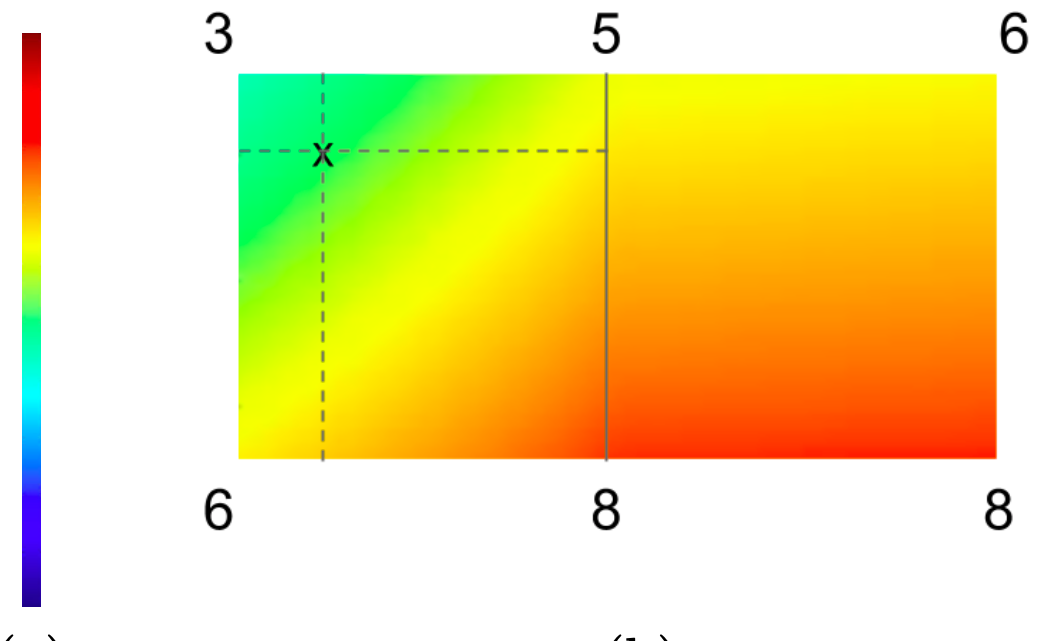
\includegraphics[width=0.5\textwidth]{img/interpol} % first figure itself
	\caption{Example for a $D = 2$ lattice function $f(x)$. Assuming (a) would be scaled with $[0, 1]$, then $f(x)$ would be approx. a value of $0.5$ \citep{gupta2016monotonic}.}
	\label{Fig:int}
\end{figure}
 Fig. \ref{Fig:int} shows the simple case of a $2 \times 2$ lattice; to evaluate the lattice function, $x$ is linearly interpolated from parameter values $\theta = (6, 8, 3, 5)$ at the vertices $v_1, v_2, v_5, v_6$. The interpolation method therefore consists of a linear combination $\phi_k(x) = [\phi_1(x), \dots \phi_{2^D}(x)]^T$ of the surrounding vertice outputs $\theta$. \citep[p.~3]{gupta2016monotonic} give a very concise graphical description of the functioning of the weighting for low dimensional cases as in Fig. \ref{Fig:int}: \begin{quote} \small
	The weights on the parameters [at the vertices] are the areas of the four boxes formed by the dotted lines drawn orthogonally through $x$, with each parameter weighted by the area of the box farthest from it, so that as $x$ moves closer to a parameter the weight on that parameter gets bigger.
\end{quote} 
To interpolate any point $x$ we first need to be able to index its surrounding lattice cell. To obtain the \textit{k}th vertex of the lattice cell, that surrounds $x$, a function $c_k(x): \mathbb{R}^{d} \rightarrow \mathbb{N}$ (for details on its computation see \citep{garcia2012optimized} is defined.  Let then $v_{c_k(x)}\ for\ (k = 1, \dots, 2^D)$ be the \textit{k}th vertex of the lattice cell containing $x$. The associated weights $\phi_k(x)$ for that cell can then be computed as
\begin{equation}
\phi_k(x) = \prod_{d=0}^{D-1} x[d]^{v_k[d]}(1- x[d])^{1-v_k[d]}.
\label{Eq:latregint}
\end{equation}
Note that we assumed a $2^D$ lattice, in this case $v_k \in \{0,1\}^D$ can be seen as the \textit{k}\ th vertex of the unit hypercube (the logic stays the same for multi-cell lattices, the formulas can be looked up in \citep{garcia2012optimized}. The exponent functions as a bitwise selector, multiplying one of the two $x[d]$ terms. We can then form the $M \times 1$ sparse weight vector for each observation $x_i$:
\begin{equation}
	\phi(x_i)[d] = \begin{cases}
	\phi_k(x_i) & \text{if } d = c_k(x_i),\ \text{for } k = 1, \dots, 2^D\\
	 \mspace{18mu} 0 &  \text{otherwise}.
	\end{cases}
\end{equation}
The function value for $x_i$ is then interpolated as $\theta^T \phi(x_i)$; concatenating all these individual vectors yields us a matrix, which can be described as the lattice function $\theta^T \phi(x)$. In addition, we can think of it as a kernel method that maps $x$ to a transformed feature vector $\phi(x)$. Garcia and Gupta chose \textit{d}-linear interpolation as method, because it can be implemented efficiently and it is the maximum entropy solution to Eq. \ref{Eq:latregsys}. \citep{gupta2016monotonic} also accredit the $\theta$ parametrization an improved interpretability effect. In addition they propose two new methods for faster interpolation (with \textit{simplex} interpolation requiring $\mathcal{O}(D log D)$ operations instead of $\mathcal{O}(D2^D)$, as with d-linear interpolation). To complete the lattice regression method we still need to supplement Eq. \ref{Eq:latregob1} with a regulizer term.

\subsubsection{Regulizer}

With the purpose to reduce over-fitting to the training data and to ensure a unique solution to Eq. \ref{Eq:latregob1} \citep{garcia2012optimized} introduce two kinds of graph regulizers $R(\theta)$. On the one hand there is the \textit{graph Laplacian} regulizer: 
\begin{equation}
	R_{laplacian}(\theta) = \sum_{adjacent\ v_r, v_s} 
	(\theta_r - \theta_s)^2 
	= \theta^T\mathbf{K}_L\theta.
	\label{Eq:latreglap}
\end{equation}
Here, the sum of squared differences between the lattice values $\theta$ at adjacent vertices $v_j$ is penalized.  Multiplying Eq. \ref{Eq:latreglap} with a regularization paramater $\lambda > 0$ (smoothness/accuracy trade off) and adding it to the regression objective of Eq. \ref{Eq:latregob1}, this yields a closed form solution $(\phi(x)^T\phi(x)^{-1} + \lambda \mathbf{K}_L)\phi(x)^T y$. %\medskip

\begin{figure}[htb]%
	\centering
	\subfloat[Laplacian]{{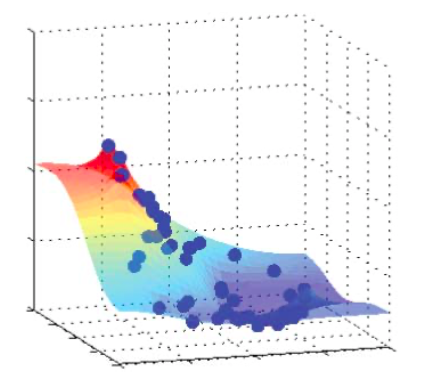
\includegraphics[height=4cm]{img/reg1} }}%
	\hspace{2cm}
	\subfloat[Hessian]{{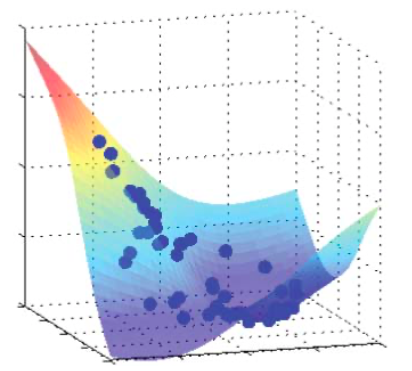
\includegraphics[height=4cm]{img/reg2} }}%
	\caption{Implementation of two regulizers on the same training data (blue dots). \citep{garcia2012optimized}}%
	\label{Fig:reg1}%
\end{figure} 

Garcia and Gupta argue that the Laplacian regulizer is not optimal, as it penalizes the estimation of linear functions. Therefore they propose a regulizer which penalizes the second-order difference in each dimension of the lattice:

\begin{equation}
		R_{hessian}(\theta) = \sum_{d=1}^{D}
		\sum_{\substack{v_r, v_s, v_t\\ adjacent\ in\\ dimension\ d}} 
		((\theta_t - \theta_r) - (\theta_r - \theta_s))^2
		= \theta^T\mathbf{K}_H\theta.
		\label{Eq:latreghes}
\end{equation}

They refer to Eq. \ref{Eq:latreghes} as \textit{graph Hessian} regulizer. In the same way as Laplacian regulizer it yields a closed form solution to \ref{Eq:latregob1}: 
\begin{equation*}
	(\phi(x)^T\phi(x)^{-1} + \lambda \mathbf{\tilde{K}}_H)\phi(x)^T y\quad \mathrm{with}\quad \tilde{K}_H = K_H + 10^{-6}\mathbf{I}. 
\end{equation*}
What is the difference to the Laplacian? Fig. \ref{Fig:reg1} shows how the Hessian regulizer permits linear extrapolations, whereas the Laplician penalizes them. 

Furthermore, \citep{gupta2016monotonic} propose a third type of regulizer; it functions in a similar way as the Hessian regulizer, making the function more linear. For a concise comparison of all three regulizers, see p. 20.\medskip 

With the regulizer at hand, the lattice regression objective has the following form:
\begin{equation}
arg\ \underset{\theta \in \mathbb{R}^{M}}{min} \sum_{i = 1}^{n} \ell(y_i, \theta^T \phi(x_i)) + R(\theta).
\label{Eq:latregob2}
\end{equation}

Regarding the credit score example from Sec. \ref{Sec:intro} the above objective function is just the base framework. To obtain the full functionality of the TFL calibrated model we will use for the experiment in Sec. \ref{Sec:Exp}, Eq. \ref{Eq:latregob2} has to be augmented with \textit{monotonicity constraints} and \textit{feature calibration}. We briefly introduce both additions in the following subsection.

%\begin{equation}
%	R_{torsion}(\theta) = \sum_{d=1}^{D}
%	                            \sum_{\substack{\tilde{d}=1\\
%	                            \tilde{d}\not= d}}^{D}\;
%	                            \sum_{\substack{r,s,t,u\ such\ that\\
%			                    v_r\ and\ v_s adjacent\ in\ dim.\ d,\\ 
%	                            v_t\ and\ v_u adjacent\ in\ dim.\ d,\\
%                                v_r\ and\ v_t adjacent\ in\ dim.\ \tilde{d}}} 
%                                ((\theta_r - \theta_s) - (\theta_t - \theta_u))^2 
%                                = \theta^T\mathbf{K}_T\theta
%\end{equation}



\subsection{Lattice Framework Extensions}

The extension of lattice regression to monotonic functions and jointly learning covariate calibration was proposed by \citep{gupta2016monotonic}. For our case study we will use a TFL linear model which is monotonically constrained and calibrated; therefore we are give a brief overview on both in the next two subsections. 

\subsubsection{Monotonicity}

For the problem setting of lattice regression Gupta et al. give the following definition for monotonicity:
\vspace*{-1cm}
\begin{quote}
	\begin{defin*}
		A function $f(x)$ is monotonically increasing with respect to feature $d$ if $f(x_i) \geq f(x_j)$ for any two feature vectors $x_i,x_j \in \mathbb{R}^D$ where $x_i[d] \geq x_j[d]$ and $x_i[m] = x_j[m]$ for $m \neq d$. 
	\end{defin*}
\end{quote}
Monotonic constraints are applied to machine learning problems to impose prior knowledge and also regularize the estimated functions. Fig. \ref{Fig:mon1} shows an example of an applied constraint. Gupta et al. give an extinsive overview of the related literature concerning the learning of monotonic functions.

For lattice regression, the goal is to ensure that a monotonic function is learned. Therefore some constraints have to be imposed on lattice output parameters $\theta$ during the learning process. For a $2^D$ lattice to be monotonically increasing in the \textit{d}th covariate Gupta et al. give the following lemma for the monotonicity constraints (p. 12):
\vspace*{-1cm}
\begin{quote}
	\begin{lemma*}
		Let $f(x) = \theta^T\phi(x)$ for $x \in [0, 1]^D$ and $\phi(x)$ given in Eq. \ref{Eq:latregint}. The partial derivative $\partial f(x)/\partial x[d] > 0$ for fixed $d$ and any $x$ iff $\theta k' > \theta k$ for all $k,k'$ such that $v_k[d] = 0, v_k'[d] = 1$ and $v_k[m] = v_k'[m]$ for all $m \neq d$. 
	\end{lemma*} 
\end{quote}
Monotonicity is established by imposing pairwise linear inequality constraints on the lattice output $\theta$: for each pair of adjacent lattice parameters $\theta_r$ and $\theta_s$ the inequality $\theta_s > \theta_r$ has to hold. As a result the estimated function increases in a certain direction, if the lattice parameters increase in that direction.

\begin{figure}[htb]%
	\centering
	\subfloat[]{{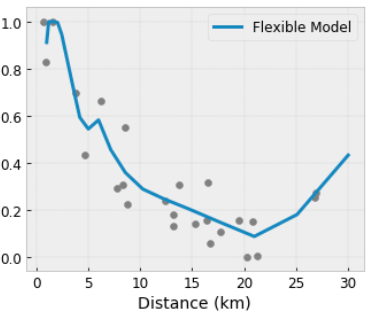
\includegraphics[height=3.5cm]{img/mon1} }}%
	\hspace{0.7cm}
	\subfloat[]{{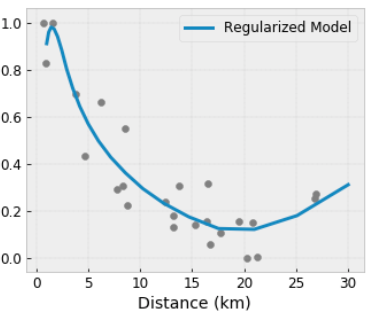
\includegraphics[height=3.5cm]{img/mon2} }}%
	\hspace{0.7cm}
	\subfloat[]{{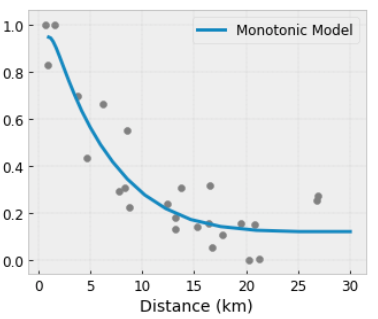
\includegraphics[height=3.5cm]{img/mon3} }}%
	\caption{The monotonic model (c) ensures that the output only decreases with respect to an input; models (a) and (b) fail in this regard (\url{https://www.tensorflow.org/lattice/overview}).}%
	\label{Fig:mon1}%
\end{figure}

To implement the constraints in the regression objective, Gupta et al. then relax strict monotonicity to monotonicity `by allowing equality in the adjacent parameter constraints' (p. 13). The updated monotonic lattice regression objective then looks the following:
\begin{align}
arg\ \underset{\theta}{min} \sum_{i = 1}^{n} \ell(y_i, \theta^T \phi(x_i)) + R(\theta)\ \mathrm{s.t.}\ A\theta \leq b.
\label{Eq:monlatreg}
\end{align}

The pairwise constraints for the lattice output $\theta$ is written as $A\theta \leq b$, whereby $A$ is a sparse matrix with one row per constraint and one $1$ and $-1$ per row. $A$ enables the specification of each individual covariate, wheter it should be constrained or unconstrained. To further constrain the fitted function in linear ways (for instance by $f(x) \geq 0$) additional linear constraints can be imposed through $A\theta \leq b$.

\subsubsection{Calibration}\label{Sec:cal}

As a way to increase accuracy, \citep{gupta2016monotonic} propose a method for transforming each covariate before they are supplied to the lattice function $f(x)$. This poses an alternative to refining the lattice by increasing the hyperparameter $M_d$, as this would be inefficient on a larger scale. \textit{Feature calibration} is an automated one-dimensional pre-processing operation $c_d[x_d]$, calibrating each of the \textit{d} covariates of $x \in D$. For continous data the authors present a one-dimensional monotonic piecewise linear function. For categorical data they propose a function for mapping each category to a real value in $[0, M_d - 1]$. Furthermore there is a suggestion of two methods to handle missing values by using a calibration approach. Now, to learn a calibrated monotonic lattice, calibration functions $c_d(\cdot)$ and lattice parameters $\theta$ are simultaneously optimized. This requires the following adjustment of the regression objective:
\begin{equation}
arg\ \underset{\theta, \alpha}{min} \sum_{i = 1}^{n} \ell(y_i, \theta^T \phi(c(x_i, \alpha))) + R(\theta)\ 
\mathrm{s.t.}\ A\theta \leq b\ \mathrm{and}\ \tilde{A}\alpha \leq b.
\label{Eq:calregobj}
\end{equation}
The vector function $c(x;\alpha)$ maps a feature vector $x$ to the lattice function $\theta^T\phi(x)$ and entails the \textit{d}th component function $c_d(x[d];\alpha^{(d)})$, which is a calibration function depending on the parameter $\alpha^{(d)}$ and the \textit{d}th component of $x$. As before $A$ denotes the monotonicity constraint, while $\tilde{A}$ does the same for each pair of adjacent calibration parameters of the calibration functions  $c(x;\alpha)$. We leave our review of lattice calibration at that. For a far more detailed description see \cite{gupta2016monotonic}; furthermore an neural network implementation (\textit{deep lattice networks}) of the theory briefly sketched in this section can be found in \citep{you2017deep}. 